\documentclass[notes=show]{beamer}
\usepackage{amsmath,amsfonts}
\usetheme{Madrid}
\usecolortheme{seagull}
\setbeamertemplate{navigation symbols}{}

\begin{document}

\title{GMM, Indirect Inference and Bootstrap}
\subtitle{Multivariate random variables and multivariate normal distribution}
\author[Willi Mutschler]{Willi Mutschler}
\date{Winter 2015/2016}
\institute{TU Dortmund}
\maketitle

\section{Multivariate random variables}
\begin{frame}\frametitle{TO IMPROVE}
  DO YOU REALLY NEED THIS???
\end{frame}
\begin{frame}\frametitle{Multivariate random variables}\framesubtitle{Random vectors}
\begin{itemize}
    \item Let
    \begin{equation*}
        X_{i}{:\Omega }\rightarrow \mathbb{R},i=1,\ldots ,n,
    \end{equation*}
    be random variables. The vector $X=(X_{1},\ldots ,X_{n})^{\prime }$ is called \textbf{random vector }or $n$-dimensional random variable
    \item Multivariate random variables are a natural generalization of univariate random variables
    \item For $n=2$ we often write $\left( X,Y\right) $ instead of $(X_{1},X_{2}) $
    \item In the following we mostly refer to the bivariate case
\end{itemize}
\end{frame}


\begin{frame}\frametitle{Multivariate random variables}\framesubtitle{Joint distribution function}
\begin{itemize}
    \item The function
        \begin{equation*}
            F_{X,Y}(x,y)=P(X\leq x,Y\leq y)
        \end{equation*}%
        for $\left( x,y\right) \in \mathbb{R}^{2}$ is called joint \textbf{cumulative distribution function} (or cdf, or distribution function) of $\left( X,Y\right)$
    \item $F_{X,Y}$ is monotonic increasing in $x$ and $y$ with limits
        \begin{eqnarray*}
            \lim_{x\rightarrow -\infty }F_{X,Y}\left( x,y\right) &=&\lim_{y\rightarrow -\infty }F_{X,Y}\left( x,y\right) =0 \\
            \lim_{x\rightarrow \infty ,y\rightarrow \infty }F_{X,Y}\left( x,y\right) &=&1
        \end{eqnarray*}
\end{itemize}
\end{frame}


\begin{frame}\frametitle{Multivariate random variables}\framesubtitle{Discrete random variables}
\begin{itemize}
    \item $(X,Y)$ are called\textbf{\ jointly discrete} if there is a finite\newline
        (or countably infinite) number of points $x_{i}$ and $y_{j}$ such that    \begin{equation*}
            P(X=x_{i},Y=y_{j})>0
        \end{equation*}
        and $\sum_{i}\sum_{j}P(X=x_{i},Y=y_{j})=1$
    \item Joint distribution function $F_{X,Y}$
    \begin{equation*}
        F_{X,Y}(x,y)=\sum_{i|x_{i}\leq x}\sum_{j|y_{j}\leq y}P(X=x_{i},Y=y_{j})
    \end{equation*}
\end{itemize}
\end{frame}



\begin{frame}\frametitle{Multivariate random variables}\framesubtitle{Continuous random variables}
\begin{itemize}
    \item $(X,Y)$ are called \textbf{jointly continuous }if there is a non-negative function $f_{X,Y}$ such that
        \begin{equation*}
            F_{X,Y}(x,y)=\int_{-\infty }^{x}\int_{-\infty }^{y}f_{X,Y}(u,v)dvdu
        \end{equation*}
    \item $f_{X,Y}$ is called the \textbf{joint density} (or pdf) of $(X,Y)$
    \item The density is
    \begin{equation*}
        f_{X,Y}(x,y)=\frac{\partial ^{2}\ F_{X,Y}(x,y)}{\partial x\partial y}
    \end{equation*}
\end{itemize}
\end{frame}


\begin{frame}\frametitle{Multivariate random variables}\framesubtitle{Density}
\begin{itemize}
    \item The volume under the density is a probability
    \item Therefore
        \begin{equation*}
            \int_{-\infty }^{\infty }\int_{-\infty }^{\infty }f\left( x,y\right) dxdy=1
        \end{equation*}
    \item The probability that $(X,Y)$ is inside the rectangle $[a,b]\times \lbrack a^{\prime },b^{\prime }]$ is
    \begin{eqnarray*}
        &&P\left( a<X\leq b,a^{\prime }<Y\leq b^{\prime }\right) \\
        &=&\int_{a}^{b}\int_{a^{\prime }}^{b^{\prime }}f_{X,Y}(u,v)dvdu
    \end{eqnarray*}
\end{itemize}
\end{frame}


\begin{frame}\frametitle{Multivariate random variables}\framesubtitle{Density}
\begin{center}
    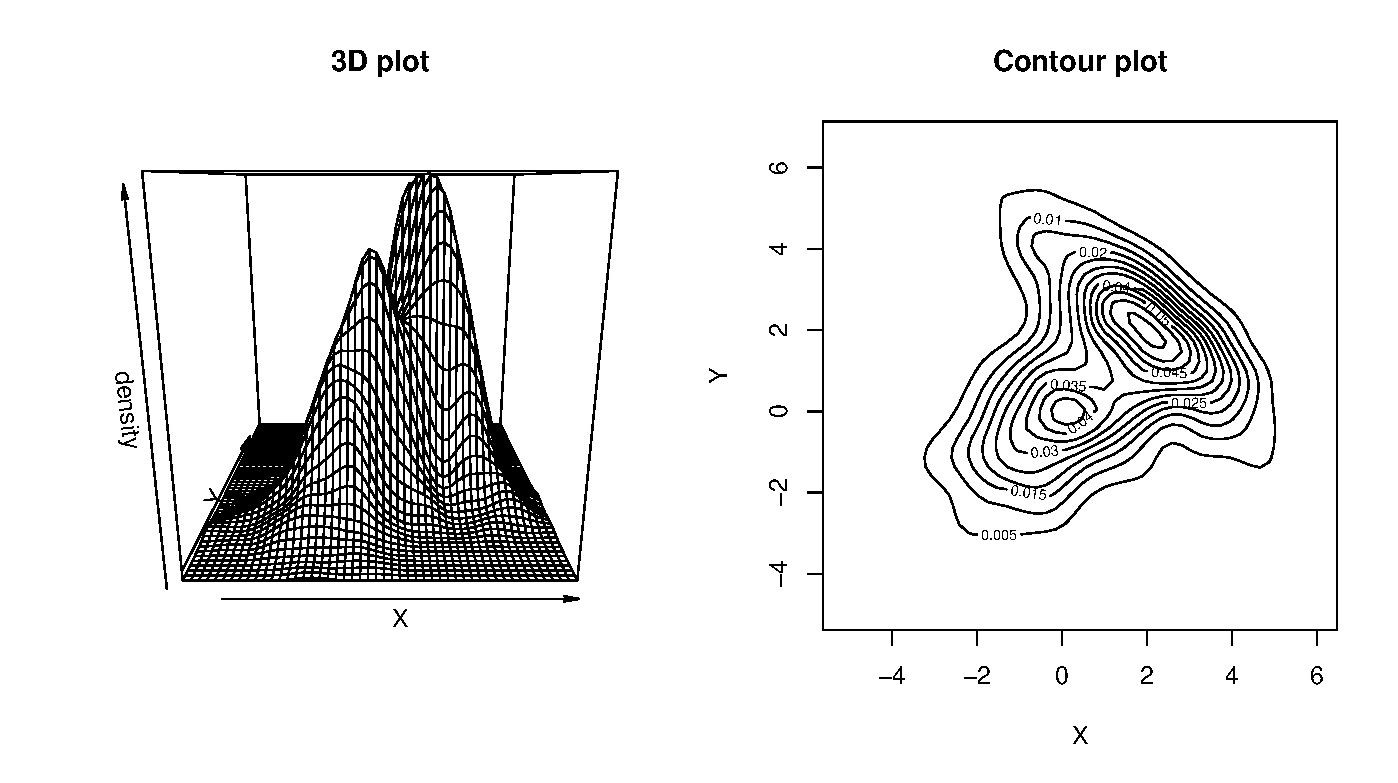
\includegraphics[width=10cm]{../plots/bvdensity.pdf}
\end{center}
\end{frame}


\begin{frame}\frametitle{Multivariate random variables}\framesubtitle{Marginal distributions}
\begin{itemize}
    \item Let $\left( X,Y\right) $ be a random vector, then%
    \begin{eqnarray*}
        F_{X}(x) &=&F_{X,Y}(x,\infty )=\lim_{y\rightarrow \infty }F_{X,Y}(x,y) \\
        F_{Y}(y) &=&F_{X,Y}(\infty ,y)=\lim_{x\rightarrow \infty }F_{X,Y}(x,y)
    \end{eqnarray*}%
    are called the \textbf{marginal distributions} of $X$ and $Y$
    \item The marginal densities of $X$ and $Y$ are
    \begin{eqnarray*}
        f_{X}(x) &=&\int_{-\infty }^{+\infty }f(x,y)dy \\
        f_{Y}(y) &=&\int_{-\infty }^{+\infty }f(x,y)dx
    \end{eqnarray*}
\end{itemize}
\end{frame}


\begin{frame}\frametitle{Multivariate random variables}\framesubtitle{Conditional distributions}
\begin{itemize}
    \item Reminder: Let $A$ and $B$ be two events (with $P(B)>0$), then%
    \begin{equation*}
        P(A|B)=\frac{P(A\cap B)}{P(B)}
    \end{equation*}
    \item Let $\left( X,Y\right) $ be jointly continuous; the \textbf{conditional density }of $X$ given $Y=y$ is
    \begin{equation*}
        f_{X|Y=y}(x)=\frac{f_{X,Y}(x,y)}{f_{Y}(y)}
    \end{equation*}
    and vice versa for $Y$ given $X=x$
\end{itemize}
\end{frame}


\begin{frame}\frametitle{Multivariate random variables}\framesubtitle{Conditional moments}
\begin{itemize}
    \item Conditional expectation, conditional cdf, and conditional variance of $X$ given $Y=y$%
    \begin{eqnarray*}
        E\left( X|Y=y\right) &=&\int_{-\infty }^{\infty }xf_{X|Y=y}(x)dx \\
        P\left( X\leq x|Y=y\right) &=&\int_{-\infty }^{x}f_{X|Y=y}(x)dx \\
        Var\left( X|Y=y\right) &=&\int_{-\infty }^{\infty }\left( x-E(X|Y=y)\right)^{2}f_{X|Y=y}(x)dx
    \end{eqnarray*}
\end{itemize}
\end{frame}


\begin{frame}\frametitle{Multivariate random variables}\framesubtitle{Independence}
\begin{itemize}
    \item Let $\left( X,Y\right) $ be a random vector; $X$ and $Y$ are called    (stochastically)\textbf{\ independent} if
    \begin{equation*}
        F_{X,Y}(x,y)=F_{X}(x)\cdot F_{Y}(y)
    \end{equation*}
    for all $(x,y)\in \mathbb{R}^{2}$.
    \item Equivalently: $X$ and $Y$ are independent if
    \begin{eqnarray*}
        F_{X|Y=y}\left( x\right) &=&F_{X}\left( x\right) \\
        F_{Y|X=x}\left( y\right) &=&F_{Y}\left( y\right)
    \end{eqnarray*}
    for all $x,y\in \mathbb{R}$
\end{itemize}
\end{frame}


\begin{frame}\frametitle{Multivariate random variables}\framesubtitle{Independence}
\begin{itemize}
    \item Jointly continuous $X$ and $Y$ are independent if for all $(x,y)\in \mathbb{R}^{2}$
    \begin{equation*}
        f_{X,Y}(x,y)=f_{X}(x)\cdot f_{Y}(y)
    \end{equation*}
    or
    \begin{eqnarray*}
    f_{X|Y=y}\left( x\right) &=&f_{X}\left( x\right) \\
    f_{Y|X=x}\left( y\right) &=&f_{Y}\left( y\right)
    \end{eqnarray*}
    \item If $X$ and $Y$ are independent and $g$ and $h$ two (measurable) functions, then $g(X)$ and $h(Y)$ are also independent
\end{itemize}
\end{frame}


\begin{frame}\frametitle{Multivariate random variables}\framesubtitle{Independence}
\begin{itemize}
    \item Generalization to $n$ random variables: The elements of the random vector are independent if for all $\left( x_{1},\ldots ,x_{n}\right) \in \mathbb{R}^{n}$
    \begin{equation*}
        F_{X_{1},\ldots ,X_{n}}\left( x_{1},\ldots ,x_{n}\right) =\prod_{i=1}^{n}F_{X_{i}}(x_{i})
    \end{equation*}
    or
    \begin{equation*}
        f_{X_{1},\ldots ,X_{n}}\left( x_{1},\ldots ,x_{n}\right)            =\prod_{i=1}^{n}f_{X_{i}}(x_{i})
    \end{equation*}
\end{itemize}
\end{frame}


\begin{frame}\frametitle{Multivariate random variables}\framesubtitle{Moments}
\begin{itemize}
    \item \textbf{Covariance} of $X$ and $Y$ (often denoted as $\sigma _{XY}$)%
    \begin{eqnarray*}
        Cov\left( X,Y\right) &=&E\left( \left[ X-E\left( X\right) \right] \left[Y-E\left( Y\right) \right] \right) \\
        &=&E(XY)-E(X)E(Y)
    \end{eqnarray*}
    \item \textbf{Correlation} of $X$ and $Y$ (often denoted as $\rho _{XY}$)%
    \begin{equation*}
        Corr\left( X,Y\right) =\frac{Cov\left( X,Y\right) }{\sqrt{Var\left( X\right)}\sqrt{Var\left( Y\right) }}
    \end{equation*}
\end{itemize}
\end{frame}


\begin{frame}\frametitle{Multivariate random variables}\framesubtitle{Moments}
\begin{itemize}
    \item \textbf{Expectation vector} of $X=\left( X_{1},\ldots ,X_{n}\right) ^{\prime }$%
        \begin{equation*}
            E\left( X\right) =\left[
            \begin{array}{c}
            E\left( X_{1}\right) \\
            \vdots \\
            E\left( X_{n}\right)
            \end{array}
            \right]
        \end{equation*}
    \item \textbf{Covariance matrix} of $X=\left( X_{1},\ldots ,X_{n}\right) ^{\prime }$%
        \begin{eqnarray*}
            Cov(X) &=&E\left[ \left( X-E(X)\right) \left( X-E(X)\right) ^{\prime }\right]\\
            &=&E(XX^{\prime })-E(X)E(X)^{\prime }
        \end{eqnarray*}
    \end{itemize}
\end{frame}


\begin{frame}\frametitle{Multivariate random variables}\framesubtitle{Moments}
Properties of covariance matrices
\begin{itemize}
    \item Symmetry: $Cov(X)=Cov(X)^{\prime }$
    \item $Cov(X)$ is positive semidefinite, i.e. for all real vectors $a\neq 0$%
        \begin{equation*}
            a^{\prime }Cov(X)a\geq 0
        \end{equation*}
    \item All diagonal elements are non-negative
    \item All eigenvalues of $Cov(X)$ are non-negative
    \item All sub-determinants are non-negative
    \end{itemize}
\end{frame}


\begin{frame}\frametitle{Multivariate random variables}\framesubtitle{Linear transformations}
\begin{itemize}
    \item Let $X=\left( X_{1},\ldots ,X_{n}\right) ^{\prime }$ be a random vector with
        \begin{eqnarray*}
            E\left( X\right) &=&\mu _{X} \\
            Cov\left( X\right) &=&\Sigma _{X}
        \end{eqnarray*}
    \item Let
        \begin{equation*}
            Y=AX+b
        \end{equation*}
        where $A$ is a real matrix and $b$ a real vector
    \item What are $E\left( Y\right) $ and $Cov\left( Y\right) $?
\end{itemize}
\end{frame}


\begin{frame}\frametitle{Multivariate random variables}\framesubtitle{Linear transformations}
\begin{itemize}
    \item The expectation vector is
        \begin{eqnarray*}
            E(Y) &=&AE(X)+b \\
            &=&A\mu _{X}+b
        \end{eqnarray*}
    \item The covariance matrix is
        \begin{eqnarray*}
            Cov(Y) &=&ACov(X)A^{\prime } \\
            &=&A\Sigma _{X}A^{\prime }
        \end{eqnarray*}
    \item Special case: If $A$ is a row vector, then $A\Sigma _{X}A^{\prime }$ is the variance of the univariate random variable $Y$
\end{itemize}
\end{frame}



\section{Multivariate normal distribution}

\begin{frame}\frametitle{Multivariate normal distribution}\framesubtitle{Outline}
\begin{itemize}
    \item Univariate standard normal distribution $N(0,1)$
    \item Univariate normal distribution $N(\mu ,\sigma ^{2})$
    \item Relation between $N(0,1)$ and $N(\mu ,\sigma ^{2})$
    \item Generalization to the $K$-dimensional case
\end{itemize}
\end{frame}


\begin{frame}\frametitle{Multivariate normal distribution}\framesubtitle{Univariate standard normal distribution}
\begin{itemize}
    \item Let $U$ be a random variable with density function
        \begin{equation*}
            \varphi \left( u\right) =\frac{1}{\sqrt{2\pi }}\exp \left( -\frac{1}{2} u^{2}\right) ,
        \end{equation*}
        then $U$ is called \textbf{standard normally (Gaussian) distributed}
    \item The distribution function $\Phi \left( u\right) =\int_{-\infty}^{u}\varphi \left( t\right) dt$ is tabulated and implemented in R etc.
    \item Moments: $E(U)=0$ and $Var(U)=1$
\end{itemize}
\end{frame}


\begin{frame}\frametitle{Multivariate normal distribution}\framesubtitle{Univariate normal distribution}
\begin{itemize}
    \item Let $X$ be a random variable with density function
        \begin{equation*}
            f\left( x\right) =\frac{1}{\sqrt{2\pi }\sigma }\exp \left( -\frac{1}{2}\left( \frac{x-\mu }{\sigma }\right) ^{2}\right) ,
        \end{equation*}
        then $X$ is called \textbf{normally (Gaussian) distributed}
    \item The distribution function is implemented in R etc.,\newline but it is not tabulated
    \item Moments: $E(X)=\mu $ and $Var(X)=\sigma ^{2}$
\end{itemize}
\end{frame}


\begin{frame}\frametitle{Multivariate normal distribution}\framesubtitle{Connections}
\begin{itemize}
    \item Let $U\sim N\left( 0,1\right) $, then $X=\mu +\sigma U\sim N(\mu,\sigma ^{2})$
    \item Let $X\sim N\left( \mu ,\sigma ^{2}\right) $, then $U=(X-\mu )/\sigma\sim N\left( 0,1\right) $
    \item Distribution functions
        \begin{equation*}
            F_{X}\left( x\right) =\Phi \left( \frac{x-\mu }{\sigma }\right)
        \end{equation*}
    \item Quantile functions
        \begin{equation*}
            x_{p}=\mu +\sigma u_{p}
        \end{equation*}
\end{itemize}
\end{frame}



\begin{frame}\frametitle{Multivariate normal distribution}\framesubtitle{K-dimensional normal distribution}
\begin{itemize}
    \item A $K$-dimensional random vector $X=\left( X_{1},\ldots ,X_{K}\right)^{\prime }$ is called \textbf{multivariate normal} with parameters
        \begin{equation*}
            \mu =\left[
            \begin{array}{c}
            \mu _{1} \\
            \vdots \\
            \mu _{K}
            \end{array}
            \right] \quad \text{und \quad }\Sigma =\left[
            \begin{array}{ccc}
            \sigma _{1}^{2} & \ldots & \sigma _{1K} \\
            \vdots & \ddots & \vdots \\
            \sigma _{K1} & \ldots & \sigma _{K}^{2}
            \end{array}
            \right]
        \end{equation*}
        if, for all $x=\left( x_{1},\ldots ,x_{K}\right) ^{\prime }\in \mathbb{R}^{K} $, the density function is
        \begin{equation*}
            f\left( x\right) =\left( 2\pi \right) ^{-\frac{K}{2}}\left( \det \Sigma \right) ^{-\frac{1}{2}}\exp \left( -\frac{1}{2}\left( x-\mu \right) ^{\prime }\Sigma ^{-1}\left( x-\mu \right) \right)
        \end{equation*}
\end{itemize}
\end{frame}


\begin{frame}\frametitle{Multivariate normal distribution}\framesubtitle{K-dimensional normal distribution}
\begin{itemize}
    \item Notation
        \begin{equation*}
            X\sim N\left( \mu ,\Sigma \right)
        \end{equation*}
    \item $\mu $\textbf{\ }is a column vector of length $K$
    \item $\Sigma $ is a non-singular, positive definite $(K\times K)$ matrix\newline
        (we exclude singular matrices for simplicity)
    \item Moments
        \begin{eqnarray*}
            E\left( X\right) &=&\mu \\
            Cov\left( X\right) &=&\Sigma
        \end{eqnarray*}
\end{itemize}
\end{frame}


\begin{frame}\frametitle{Multivariate normal distribution}\framesubtitle{Properties}
\begin{itemize}
    \item Marginal distributions of $X$ are normal: If
        \begin{equation*}
            \left(
            \begin{array}{c}
            X_{1} \\
            X_{2}
            \end{array}
            \right) \sim N\left( \left[
            \begin{array}{c}
            \mu _{1} \\
            \mu _{2}
            \end{array}
            \right] ,\left[
            \begin{array}{cc}
            \Sigma _{11} & \Sigma _{12} \\
            \Sigma _{21} & \Sigma _{22}
            \end{array}
            \right] \right)
        \end{equation*}
        then
        \begin{eqnarray*}
            X_{1} &\sim &N\left( \mu _{1},\Sigma _{11}\right) \\
            X_{2} &\sim &N\left( \mu _{2},\Sigma _{22}\right)
        \end{eqnarray*}
    \item \textbf{Attention}: Even if all elements are normal, the vector need not be multivariate normal!
\end{itemize}
\end{frame}


\begin{frame}\frametitle{Multivariate normal distribution}\framesubtitle{Properties}
\begin{itemize}
    \item Conditional distributions are normal,
        \begin{eqnarray*}
            X_{1}|\left( X_{2}\!=\!x_{2}\right) \!\! &\sim &\!\!N\left( \mu_{1}\!+\!\Sigma _{12}\Sigma _{22}^{-1}\left( x_{2}\!-\!\mu _{2}\right),\Sigma _{11}\!-\!\Sigma _{12}\Sigma _{22}^{-1}\Sigma _{21}\right) \\
            X_{2}|\left( X_{1}\!=\!x_{1}\right) \!\! &\sim &\!\!N\left( \mu_{2}\!+\!\Sigma _{21}\Sigma _{11}^{-1}\left( x_{1}\!-\!\mu _{1}\right),\Sigma _{22}\!-\!\Sigma _{21}\Sigma _{11}^{-1}\Sigma _{12}\right)
        \end{eqnarray*}
    \item Linear transformations are normal: If $X\sim N\left( \mu ,\Sigma\right) ,$ then
        \begin{equation*}
            AX+b\sim N\left( A^{\prime }\mu +b,A^{\prime }\Sigma A\right)
        \end{equation*}
\end{itemize}
\end{frame}



\begin{frame}\frametitle{Multivariate normal distribution}\framesubtitle{Properties}
\begin{itemize}
    \item Let $X\sim N\left( \mu ,\Sigma \right) $ with $\Sigma $ positive definite, then there is a matrix $V$, such that
        \begin{equation*}
            \Sigma =VV^{\prime }
        \end{equation*}
        and
        \begin{equation*}
            X=\mu +VU
        \end{equation*}
        where
        \begin{equation*}
            U\sim N\left( 0,I\right)
        \end{equation*}
\end{itemize}
\end{frame}


\begin{frame}\frametitle{Multivariate normal distribution}\framesubtitle{Markowitz portfolio theory}
\begin{itemize}
    \item Let $X\sim N\left( \mu ,\Sigma \right) $ be the vector of returns of $K $ assets
    \item Let $A$ be a $\left( 1\times K\right) $ row vector of portfolio weights
    \item Portfolio return $Y=AX$ (scalar)
    \item The portfolio return is normally distributed,
        \begin{equation*}
            Y\sim N\left( A\mu ,A\Sigma A^{\prime }\right)
        \end{equation*}
\end{itemize}
\end{frame}
\end{document} 